\documentclass[12pt,twoside]{report}
\usepackage[a4paper,hmargin=2.5cm,vmargin=2.5cm,includeheadfoot]{geometry}

\newcommand{\reporttitle}{Wisent++: A C++ Library for Composability-Enabled Data File Formats}
\newcommand{\reportauthor}{Amor Zhao}
\newcommand{\supervisor}{Dr Holger Pirk}
\newcommand{\secondmarker}{Dr Marios Kogias}
\newcommand{\reporttype}{MEng Individual Project \\ Interim Report}
\newcommand{\cid}{02019680}

\usepackage{colortbl}
\usepackage{ifxetex}
\usepackage{textpos}
\usepackage{stackengine}
\usepackage{tabularx,longtable,multirow,subfigure,caption}
\usepackage{fancyhdr}
\usepackage[bottom]{footmisc}
\usepackage[tight,ugly]{units}
\usepackage{url}
\usepackage{float}
\usepackage[english]{babel}
\usepackage{amsmath}
\usepackage{graphicx}
\usepackage[colorinlistoftodos]{todonotes}
\usepackage{epstopdf} % automatically replace .eps with .pdf in graphics
\usepackage{array}
\usepackage{latexsym}
\usepackage{etoolbox}
\usepackage{enumerate} 
\usepackage{tcolorbox}
\usepackage{kpfonts}
\usepackage{csquotes}
\usepackage[style=vancouver,backend=biber]{biblatex}
\addbibresource{Bibliography/references.bib}
\usepackage{afterpage}

\newcommand{\fig}[3]{
 \begin{center}
 \scalebox{#3}{\includegraphics[#2]{#1}}
 \end{center}
}

% Define a tcolorbox style for pseudocode
\tcbuselibrary{listingsutf8} % Ensure compatibility with code listings
\tcbset{
  pseudocodebox/.style={
    colframe=black,
    colback=white,
    coltitle=black,
    colbacktitle=white,
    fonttitle=\bfseries,
    boxrule=0.5mm, 
    width=\textwidth,
    sharp corners,
    left=1mm,
    right=1mm,
    bottom=1mm,
    top=1mm
  }
}

\ifxetex
\usepackage{fontspec}
\setmainfont[Scale=.8]{OpenDyslexic-Regular}
\else
\usepackage[pdftex,pagebackref=false,hypertexnames=false,colorlinks]{hyperref}
\hypersetup{pdftitle={},
  pdfsubject={}, 
  pdfauthor={\reportauthor},
  pdfkeywords={}, 
  pdfstartview=FitH,
  pdfpagemode={UseOutlines},% None, FullScreen, UseOutlines
  bookmarksnumbered=true, bookmarksopen=true, colorlinks,
    citecolor=darkgray,
    filecolor=darkgray,
    linkcolor=black,
    urlcolor=darkgray}
\usepackage[all]{hypcap}
\fi

\usepackage{setspace}
\setlength\parskip{\baselineskip}
\setlength{\parskip}{1.5ex}  % Space between paragraphs
\usepackage{enumitem}

% ========================================================================

\begin{document}

\ifxetex
\else
\renewcommand*{\rmdefault}{bch} % Charter
\renewcommand*{\ttdefault}{cmtt} % Computer Modern Typewriter
\fi

\setlength{\parindent}{2em}  % indentation of paragraph
\setlength{\headheight}{14.5pt}

\fancypagestyle{contentstyle}{
  \fancyhf{}
  \renewcommand{\headrulewidth}{0pt}
  \renewcommand{\footrulewidth}{0pt}
  \fancyfoot[]{}
}

\fancypagestyle{chapterstyle}{
  \fancyhf{}
  \renewcommand{\headrulewidth}{0pt}
  \renewcommand{\footrulewidth}{0.1pt}
  \fancyfoot[ER,OL]{\thepage}
}

\defbibheading{bibliography}[\refname]{
  \chapter*{Bibliography}
  \thispagestyle{chapterstyle}
  \addcontentsline{toc}{chapter}{#1}  
  \pagestyle{fancy} % Apply fancy page style for subsequent pages
  \markboth{\MakeUppercase{BIBLIOGRAPHY}}{}
}

\let\origfootrule\footrule
\renewcommand{\footrule}{\iffootnote{}{\origfootrule}}
\renewcommand\footnoterule{\origfootrule \vspace{1ex}}

% various color definitions
\definecolor{darkgreen}{rgb}{0,0.6,0}
\newcommand{\blue}[1]{{\color{blue}#1}}
\newcommand{\red}[1]{{\color{red}#1}}
\newcommand{\green}[1]{{\color{darkgreen}#1}}
\newcommand{\orange}[1]{{\color{orange}#1}}
\newcommand{\magenta}[1]{{\color{magenta}#1}}
\newcommand{\cyan}[1]{{\color{cyan}#1}}

% redefine emph
\renewcommand{\emph}[1]{\blue{\bf{#1}}}

% place a colored box around a character
\gdef\colchar#1#2{
  \tikz[baseline]{
    \node[anchor=base,inner sep=2pt,outer sep=0pt,fill = #2!20] {#1};
  }
}

%% ========================================================================

% title page
\newgeometry{left=2.4cm, right=2.4cm, top=3.5cm, bottom=2.5cm}
\begin{titlepage}

\newcommand{\HRule}{\rule{\linewidth}{0.5mm}} 

%----------------------------------------------------------------------------------------
%	LOGO SECTION
%----------------------------------------------------------------------------------------

\hspace{-0.6cm} 

\includegraphics[width=8cm]{./Figures/imperial-new-logo.png}\\[0.5cm]
\vspace{2cm}

\begin{center} % Center remainder of the page

%----------------------------------------------------------------------------------------
%	HEADING SECTIONS
%----------------------------------------------------------------------------------------
\fontfamily{ptm}\selectfont\textsc{\LARGE \reporttype \\[0.2cm]}
\vspace{1.3cm}
\fontfamily{ptm}\selectfont\textsc{\Large Department of Computing}\\[0.5cm] 
\fontfamily{ptm}\selectfont\textsc{\large Imperial College of Science, Technology and Medicine}\\[0.5cm] 
%----------------------------------------------------------------------------------------
%	TITLE SECTION
%----------------------------------------------------------------------------------------
\HRule \\[0.2cm]
{ \setlength{\baselineskip}{1.2\baselineskip}
    \huge \bfseries \reporttitle \\[0.3cm]}
\HRule \\[1.5cm]
\end{center}

%----------------------------------------------------------------------------------------
%	AUTHOR SECTION
%----------------------------------------------------------------------------------------

\centering
\begin{minipage}{0.5\textwidth}
\begin{flushleft} \large
\textit{Author:}\\
\reportauthor~(CID: \cid)
\end{flushleft}
\end{minipage}
~
\begin{minipage}{0.4\textwidth}
\begin{flushright} \large
\textit{Supervisor:} \\
\supervisor \\
\vspace{0.5cm}
\textit{Second Marker:} \\
\secondmarker
\end{flushright}
\end{minipage}\\[2cm]
\makeatother

\vspace{2cm}
\makeatletter
\@date 
\vfill
\makeatother

% \restoregeometry

\end{titlepage}


\restoregeometry

% table of contents
\pagestyle{contentstyle}
\addtocontents{toc}{\protect\thispagestyle{contentstyle}}
\tableofcontents 
\clearpage{\pagestyle{empty}}

% reset page numbering styles
\pagenumbering{arabic}
\setcounter{page}{1}
\fancyhead[LE,RO]{\slshape \rightmark}
\fancyhead[LO,RE]{\slshape \leftmark}
\clearpage{\pagestyle{empty}\cleardoublepage}
\setlength{\headheight}{14.5pt}
\pagestyle{fancy}

\renewcommand{\chaptermark}[1]{\markboth{\chaptername\ \thechapter.\ \MakeUppercase{#1}}{}} 
\renewcommand{\sectionmark}[1]{\markright{\thesection.\ #1}}
\fancyfoot[ER,OL]{\thepage}
\fancyfoot[OC,EC]{\sffamily }
\renewcommand{\headrulewidth}{0.1pt}
\renewcommand{\footrulewidth}{0.1pt}
\captionsetup{margin=10pt,font=small,labelfont=bf}


%--- chapter heading
\def\@makechapterhead#1{%
  \vspace*{10\p@}%
  {\parindent \z@ \raggedright \sffamily
    \interlinepenalty\@M
    \Huge\bfseries \thechapter \space\space #1\par\nobreak
    \vskip 30\p@
  }}

%---chapter heading for \chapter*  
\def\@makeschapterhead#1{%
  \vspace*{10\p@}%
  {\parindent \z@ \raggedright
    \sffamily
    \interlinepenalty\@M
    \Huge \bfseries  #1\par\nobreak
    \vskip 30\p@
  }}	
\allowdisplaybreaks

%====================================================================================================
% The aim of the project interim report is multi-fold:

% 1. To provide a document that your second marker can use as a basis for discussion on your project plan and progress to date.
% 2. To show that you have considered the ethical implications of your project.
% 3. To provide a substantial body of text, primarily the project background and related work, that you can use in your final report. 

% By the time the interim report is due you should have a clearly defined project, understand well the motivation and issues to be addressed, know the background work in detail, have the main ideas for how to tackle the problem and have started the development. You should also have a plan for the remainder of the project and, importantly, how to evaluate the project.

% The interim report should contain the following sections. An approximate page count is suggested for each section, but there are no hard limits either way:
%====================================================================================================

% ----------------- Introduction (1-3 pages) -----------------

% It’s a good idea to _try_ to write the introduction to your final report early on in the project. However, you will find it hard, as you won’t yet have a complete story and you won’t know what your main contributions are going to be. However, the exercise is useful as it will tell you what you _don’t_ yet know and thus what questions your project should aim to answer. 

% For the interim report this section should be a short, succinct, summary of the project’s main objectives. Some of this material may be re-usable in your final report, but the chances are that your final introduction will be quite different. You are therefore advised to keep this part of the interim report short, focusing on the following questions: 

% What is the problem, 
% why is it interesting 
% and what’s your main idea for solving it?  

% (DON'T use those three questions as subheadings however!  The answers should emerge from what you write.)
% -------------------------------------------------------------

\chapter{Introduction}
\thispagestyle{chapterstyle}

\section{Project Motivation}

File formats differ greatly in modern data management systems. Various data structures, file formats and compression algorithms available for managing and exchanging data makes it a growing challenge for data systems to efficiently handle diverse data models. They face the challenge of either continuously investing resources to support new file formats or restricting users to a limited selection, which may negatively impact performance and compatibility. Additionally, file formats are tightly coupled with the data they represent, meaning that any change to the data model or compression method often necessitates modifying the file format itself.

When exchanging between flat data and nested data, such discrepancy leads to inefficiencies when converting between the two, as it requires additional steps to flatten nested data or reconstruct hierarchies from flat formats, and has become a major challenge to the interprocess communication efficiency. 

With the approach of storing all data in a single file, we are able to simplify the problem of formats integration, however, it also increases processing costs. This is because parsers must treat every node as if it has children, even though many nodes may not. In this way, we change our focus to how we can efficiently store and exchange leafy trees.

The Wisent library \cite{mohr2023wisent} provides a new exchange file format which supports CPU-efficient encoding and decoding of these leafy trees. It guarantees efficient serialisation, deserialisation and in-place processing, and supports selective access to specific parts of data in the file, which allows manipulating various data structures without being constrained by specific file format designs. 

While Wisent shows better runtime performance and lower memory usage than other popular file formats like Json\cite{json_org}, Bson\cite{bson_specification}, and RapidJson\cite{rapidjson}, it does not support any data compression techniques. In comparison, other columnar data storage formats, like Parquet\cite{apache_parquet}, support various data compression schemas that allow users to easily create efficient storage and retrieval. 

With this motivation, we aim to design and build an advanced version of the Wisent C++ library, which adapts effective data compressing algorithms, while keeping Wisent's advantage of efficient selective loading and random access. 

\section{Design Objectives}

Wisent++ is designed to extend the state-of-the-art file formats to provide a flexible and efficient solution for managing and exchanging data between diverse data models, while supporting various compression schemas in modern data systems. The library should extend the five objectives of Wisent, which, as stated in the Wisent paper, includes: Nested data representation; Minimizing storage overhead; Efficient serialisation usages; Selective access and being simple to implement parser using the popular programming languages. 

In our project, we add a few more features in addition to these properties. The library should also support a variety of data compression algorithms, from the simpler algorithms like RLE, Delta encoding and LZW, to the modern (and more complicated) ones like BZip2, prediction by partial matching, etc.\cite{gupta2017modern} So, we added the following objectives in this project:

\begin{itemize}[label=\textbullet, topsep=0pt] 
\item We aim to design the library with encapsulated methods such that these algorithms could be applied efficiently and easily. 

\item Another necessary goal is to make Wisent++ adapt to current industrial need. It has been designed to build under a lowest requirement of C++ version 14, in order to best support most projects while dismissing a reasonable amount of C++ features.

\item Although it is users' freedom to choose the compression algorithm in real applications, we aim to optimise the worst case scenario during the design. 
\end{itemize}


\newpage


% ----------------- Background (10- 20 pages) -----------------

% This should form the bulk of the interim report. You should consider that your objective here is to produce a near final version of the background section, as it will appear in your final report. All of this material should be re-usable, so it is worth getting it right at this stage of the project. 

% This section of the report should set the project into context by relating it to existing published work that you read at the start of the project when your approach and methods were being considered. There are usually many ways of approaching a given problem, and you should not just pick one at random. Describe and evaluate as many alternative approaches as possible. The published work will usually be in the form of research papers, but you may also consider text books, technical manuals, or even existing software or hardware of which you have had hands-on experience. Acknowledge the sources of your inspiration; you are expected to have seen and thought about other people's ideas, so your contribution largely will be putting them into practice in some other context.

% The details of what to include can be found in the [Project Report guidelines](https://wiki.imperial.ac.uk/display/docteaching/Project+Report).
% -------------------------------------------------------------

\chapter{Background}
\thispagestyle{chapterstyle}

In this chapter, we provide an overview of some existing solutions and their compression algorithms. 

We will then take a look into the basic design principles and implementations of the Wisent file format, and explore our approaches to extend the Wisent library to support some of the popular modern compression algorithms. 

\section{Relavant Data File Types}

\subsection{Flat Data}

Flat data indicates the type of data without an embedded structure. Because of its simplicity and compatibility, files with such data formats are commonly used in databases and spreadsheets. \texttt{csv}, \texttt{tsv} and \texttt{txt} files \cite{csv_format} are some of the most common examples to store flat data. 

As illustrated in Figure. \ref{fig:flat_data_file}, the \texttt{csv} file is organised in a tabular format where each row corresponds to a record and each column corresponds to a field.

\subsection{Nested Data}

Nested data, on the other hand, is the type of data that contains an embedded structure, some typical examples includes \texttt{JSON}, \texttt{XML}, and \texttt{YAML} files\cite{json_org}. These files are commonly used to represent hierarchical data structures, such as trees, graphs, and other complex data models.

Figure. \ref{fig:nested_data_file} shows an example of a nested data file in \texttt{JSON} format. 

\begin{center}
\begin{figure}[ht]
\centering
\begin{minipage}[t]{0.44\textwidth}
\centering
\setlength{\fboxsep}{4pt}
\fbox{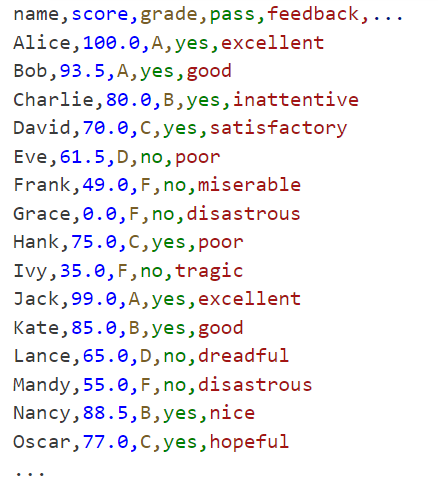
\includegraphics[height=7cm]{./Figures/flatDataExample.png}}
\caption{\centering Flat data example \newline (\texttt{student-exam-feedbacks.csv})}
\label{fig:flat_data_file}
\end{minipage}
\hfill
\begin{minipage}[t]{0.52\textwidth}
\centering
\setlength{\fboxsep}{4pt}
\fbox{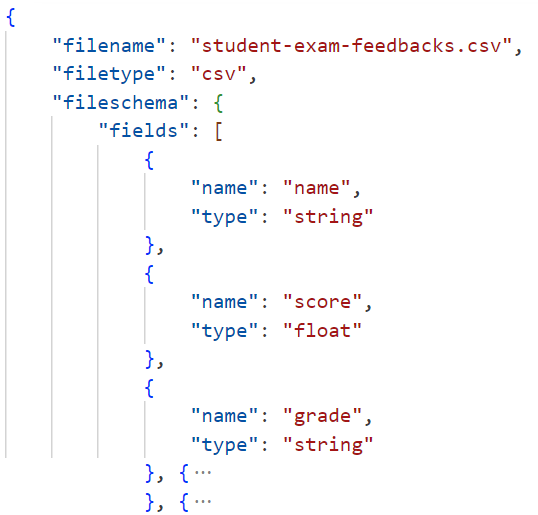
\includegraphics[height=7cm]{./Figures/nestedDataExample.png}}
\caption{\centering Nested data example \newline (\texttt{student-exam-feedbacks.json})}
\label{fig:nested_data_file}
\end{minipage}
\end{figure}
\end{center}

\subsection{Leafy Data}

In many real-world scenarios, data is stored as a combination of both flat and nested data, where a nested data file is used to represent the structure of the dataset, such as column names, data types, and other information about the flat data file, and the flat data file contains the actual tabular data. We call this type of data structure a leafy tree, where each node is either a leaf or an inner node. 

In our example of Figure. \ref{fig:flat_data_file} and \ref{fig:nested_data_file}, the flat data file contains the actual exam feedback data, while the nested data file contains the metadata about the flat data file structures. It may also be forming a bigger tree structure, where many flat data files are referenced by various nested data files like \texttt{student-exam-feedbacks.json}.


\section{Existing Solutions}

Many existing solutions for managing leafy data files are based on traditional data decomposition schemas, which store the data in a depth-first manner. We will look at some of the popular file formats here, dealing with either flat or nested data.  

\subsection{JSON}

JSON is a common text-based format for nested data serialisation, easily integrated into any language but with high serialisation costs. Several libraries, including NLohmann JSON \cite{nlohmann_json}, RapidJSON \cite{rapidjson}, and Simd-Json\cite{langdale2019parsing}, provide efficient JSON parsing and serialisation. However, JSON's text-based nature also makes it less efficient for large datasets, as it requires more storage space and processing power.

\subsection{Parquet}

The Apache Paquet file format \cite{apache_parquet} represents an advanced approach to data storage and transfer, with its compression properties playing a critical role in its overall efficiency. It employs a sophisticated compression algorithm that dynamically adapts to the characteristics of the data being compressed. This adaptive compression scheme is a cornerstone of the Paquet format's efficiency, as it minimizes both the space required for storage and the time needed for decompression. 

Paquet allows users to choose from multiple compression algorithms, including: Snappy, Gzip, Brotli, LZO, and Zstandard (Zstd). The choice of compression algorithm can significantly impact the performance of the Paquet format, as Paquet applies different trade-offs between compression ratio and speed.


\section{Basic Wisent File Format}

We now move on to the basic design principles and implementations of the Wisent file format.

As discussed in the last section, we found that one of the major drawbacks of the traditional data decomposition schema is that it requires reading the entire data structure before accessing a specific part of data, which is particularly inefficient when only a small portion of the data is needed. As long as data is stored in a depth-first manner, the structure of leafy file is unpredictable. 

Wisent, on the other hand, stores the data in a breadth-first manner, which allows efficient selective loading and random access, as we don't need to read the entire file to get the data structure. 

\subsection{Design Principles}

Figure. \ref{fig:Wisent_structure} illustrates the Wisent structure for storing a tree node. The Wisent serialisation format is divided into four distinct sections: the Argument Vector, the Type Bytefield, the Structure Vector, and the String Buffer. These components work together to store and represent the serialized data efficiently.

\begin{center}
\begin{figure}[ht]
\centering
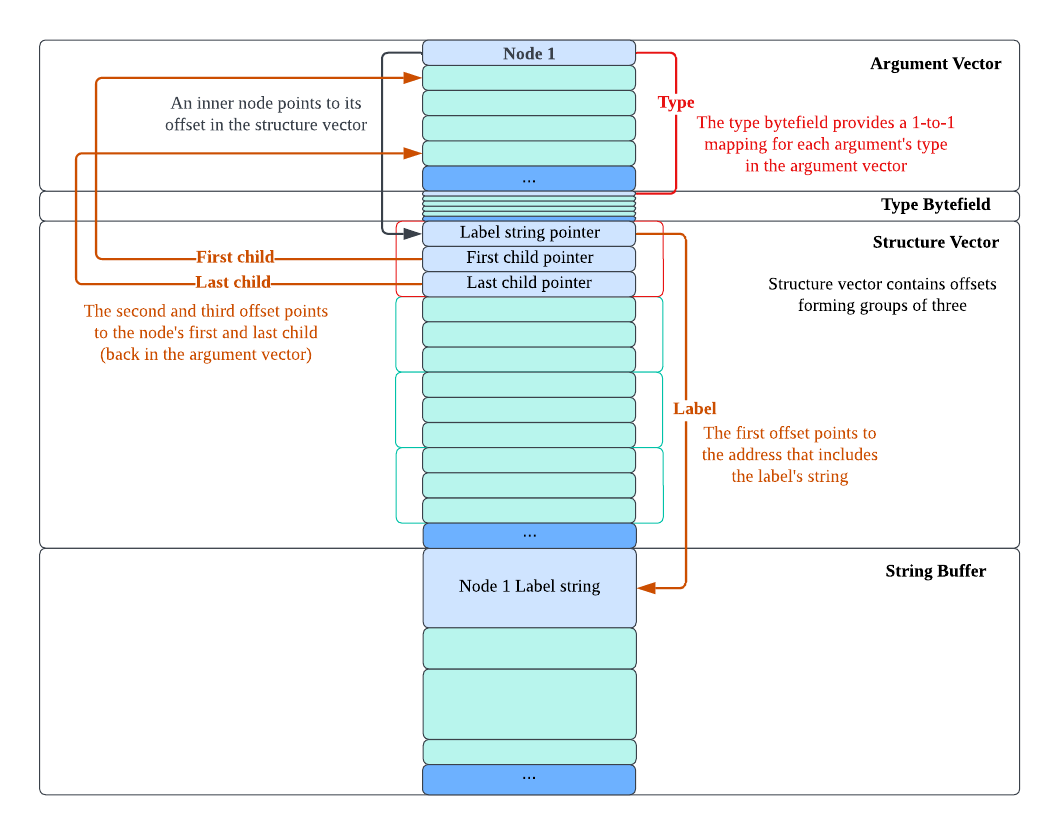
\includegraphics[width=\textwidth]{./Figures/WisentStructure.png}
\caption{Wisent structure for storing a tree node}
\label{fig:Wisent_structure}
\end{figure}
\end{center}

We take the light blue blocks as an example: 

``Node 1" represents a node argument in the tree. The Type Bytefield at this index contains a 8-bit Argument Type value ``5", indicating this argument in the Argument Vector to be an expression. The 3 corresponding offsets in the Structure Vector contains the information of its structual relationships. The first pointer points to a string in the String Buffer, while the second and third pointers point to the beginning and end of the following child nodes of ``Node 1". 

Together, they representes all the information of the node in the tree. 

For non-node arguments, the argument value is directly stored in the Argument Vector, for example, numbers as \texttt{int} or \texttt{float} types, and strings as a direct offset pointing to the String Buffer section.

\subsection{Serialisation and Deserialisation Mechanism}

The Wisent library provides a simple and efficient mechanism for serializing and deserializing data. As shown in Figure\ref{fig:serialiser} and \ref{fig:deserialiser}, the serialisation process converting the leafy data into a Wisent file, while the deserialisation process involves converting the Wisent file back into the original leafy data.

\begin{figure}[ht]
\centering
\begin{minipage}[t]{0.47\textwidth}
\begin{tcolorbox}[pseudocodebox, title=Mechanism: Wisent Serialiser]
\begin{verbatim}
Input: Leafy source data
Output: Serialised Wisent file

1. Iterate through the 
   datapackage to count 
   number of arguments
2. Allocate memory for 
      Argument Vector, 
      Type Bytefield, 
      Structure Vector, 
      and String Buffer
3. For each node in the
   datapackage, 
   serialise the node
\end{verbatim}
\end{tcolorbox}
\caption{Wisent Serialiser}
\label{fig:serialiser}
\end{minipage}%
\hfill
\begin{minipage}[t]{0.47\textwidth}
\begin{tcolorbox}[pseudocodebox, title=Mechanism: Wisent Deserialiser]
\begin{verbatim}
Input: Wisent file
Output: Deserialised data / 
        selected columnar data

1. Load the Wisent data file
2. Split the file into 
      Argument Vector, 
      Type Bytefield, 
      Structure Vector, 
      and String Buffer
3. For each node in the 
      Structure Vector, 
      reconstruct the tree
   Or lazy loads the 
      selected columnar data
\end{verbatim}
\end{tcolorbox}
\caption{Wisent Deserialiser}
\label{fig:deserialiser}
\end{minipage}
\end{figure}

We can test the performance of basic Wisent library through a series of benchmarks. The results show that Wisent outperforms other popular serialisation formats, such as JSON, BSON, and RapidJSON, in terms of both runtime performance and memory usage. The benchmarks demonstrate that Wisent is capable of serializing and deserializing data structures efficiently, making it a suitable choice for applications that require high-performance data processing.



\subsection{Approaches of Extending Wisent for Compression}

Since the Wisent library does not currently support data compression, in this project, we aim to extend the Wisent library to support various data compression algorithms.

\begin{figure}[ht]
\centering
\begin{minipage}[t]{0.47\textwidth}
\begin{tcolorbox}[pseudocodebox, title=Algorithm: Delta Encoding]
\begin{verbatim}
Input: data[]
Output: encoded[]

1. Initialize encoded[] 
   with the same size as data[]
2. Set encoded[0] = data[0]
3. For i from 1 to length of 
   data[] - 1 do
4.    encoded[i] = 
         data[i] - data[i - 1]
5. End For
6. Return encoded[]
\end{verbatim}
\end{tcolorbox}
\caption{Delta Encoding}
\label{fig:delta_encoding}
\end{minipage}%
\hfill
\begin{minipage}[t]{0.47\textwidth}
\begin{tcolorbox}[pseudocodebox, title=Algorithm: Run-Length Encoding]
\begin{verbatim}
Input: data[]
Output: encoded[]

1. Initialize encoded[] 
   with an empty list
2. Set count = 1
3. For i from 1 to length of 
   data[] - 1 do
4.    Count for the same 
      element, increment count
5.    encoded[] is appended 
      with (count, data[i - 1])
6. End For
7. Return encoded[]
\end{verbatim}
\end{tcolorbox}
\caption{Run-Length Encoding}
\label{fig:run_length_encoding}
\end{minipage}
\end{figure}

Figure. \ref{fig:delta_encoding} and \ref{fig:run_length_encoding} presents the pseudocode for two simple and popular compression algorithms: Delta Encoding and Run-Length Encoding\cite{gopinath2020comparison}. These algorithms are easy to implement and can provide significant compression ratios for certain types of data. 

The Wisent library implements run-length encoding as a built-in feature for its Type Bytefield, which can be enabled by setting a threshold in the Wisent helper library. It was designed in a runtime performance perspective, in order to reduce the time of referring to the argument type, rather than to save the storage space, though. 

Some other modern compression algorithms, including BZip2, LZW, and Prediction by Partial Matching \cite{gupta2017modern}, are more complex and require additional considerations for integration with the Wisent data processing mechanism. We may apply them in separate approaches in the string buffer and argument vectors. 



\newpage



% ----------------- Project Plan (1-2 pages) -----------------

% You should explain what needs to be done in order to complete the project and roughly what you expect the timetable to be. Don’t forget to include the project write-up (the final report), as this is a major part of the exercise. 

% It’s important to identify key milestones and also fall-back positions, in case you run out of time. You should also identify what extensions could be added if time permits. The plan should be complete and should include those parts that you have already addressed (make it clear how far you have progressed at the time of writing).  

% This material will _not_ appear in the final report.
% -------------------------------------------------------------

\chapter{Project Plan}
\thispagestyle{chapterstyle}

\section{Timeline}

The project plan (as shown in Table \ref{tab:project_plan} and \ref{tab:project_plan_2}) outlines the timeline and key milestones. The ``planned work" column shows the detailed tasks we focus on during each time period, and the ``key milestones" column states the deliverables or objectives to be achieved by the end of that period. 

\begin{table}[h!tb]
\centering
\renewcommand{\arraystretch}{1.5}
\begin{tabular}{|c|c|>{\raggedright\arraybackslash}p{5.5cm}|>{\raggedright\arraybackslash}p{3.5cm}|} \hline  

\multicolumn{1}{|c|}{\textbf{Timeline}} & \multicolumn{1}{|c|}{\textbf{Week}} & \multicolumn{1}{|c|}{\textbf{Planned Work}} & \multicolumn{1}{|c|}{\textbf{Key Milestones}} \\ \hline  

Beginning of Nov.& 1& Meet supervisor. & N/A\\ \hline  

11\textsuperscript{th} Nov. - 8\textsuperscript{th} Dec.& 2 - 5& Develop understanding of the basic Wisent design. \newline Study the Wisent test code. \newline Reproduce test results of the benchmarks.& Set up a test codebase with basic Wisent features by the beginning of Dec.\\ \hline  

\rowcolor{gray!20}
9\textsuperscript{th} Dec. - 15\textsuperscript{th} Dec.& 6& \multicolumn{2}{|c|}{Autumn term final exams}\\ \hline  

16\textsuperscript{th} Dec. - 19\textsuperscript{th} Jan.& 7 - 11& Study the state-of-the-art modern data compression algorithms and applications. \newline Explore possible ways of compression implementation. & Complete interim report by 23\textsuperscript{rd} Jan.\\ \hline 

20\textsuperscript{th} Jan. - 9\textsuperscript{th} Feb.& 12 - 13& Review the project plan and evaluation plan. \newline Make necessary changes. & Review project with second marker by 6\textsuperscript{th} Feb. \\ \hline 

\end{tabular}
\caption{Project plan}
\label{tab:project_plan}
\end{table}

\afterpage
{
   \begin{table}[h!tb]
   \centering
   \renewcommand{\arraystretch}{1.5}
   \begin{tabular}{|c|c|>{\raggedright\arraybackslash}p{5.5cm}|>{\raggedright\arraybackslash}p{3.5cm}|} \hline   

   \multicolumn{1}{|c|}{\textbf{Timeline}} & \multicolumn{1}{|c|}{\textbf{Week}} & \multicolumn{1}{|c|}{\textbf{Planned Work}} & \multicolumn{1}{|c|}{\textbf{Key Milestones}} \\ \hline  

   10\textsuperscript{th} Feb. - 23\textsuperscript{rd} Mar.& 14 - 19& Develop and integrate advanced compression algorithms. \newline Continuously perform unit testing and performance evaluations throughout the development process. & The expected performance metrics should be well-defined by this time. \\ \hline  

   24\textsuperscript{th} Mar. - 13\textsuperscript{th} Apr.& 20 - 22& Test performance on various datasets, analyse the approaches. & Our initial evaluation results should meet the expectations. \\ \hline

   14\textsuperscript{th} Apr. - 27\textsuperscript{th} Apr.& 23 - 24& Identify the performance bottle-neck, explore possible walk throughs for the performance restrictions. & We aim to finish the algorithm implementation by the start of summer term. \\ \hline

   \rowcolor{gray!20}
   28\textsuperscript{th} Apr. - 11\textsuperscript{th} May.& 25 - 26& \multicolumn{2}{|c|}{Summer term final exams}\\ \hline  

   12\textsuperscript{th} May. - 31\textsuperscript{st} May.& 27 - 29& Finish evaluation and write final report. \newline Wrap up project and clean documentations. & All necessary design objectives should be met by the start of Jun. \\ \hline  

   1\textsuperscript{st} Jun. - 13\textsuperscript{th} Jun. & 30 - 31& \multicolumn{2}{|c|}{Complete final report.}\\ \hline 

   14\textsuperscript{th} Jun. - 24\textsuperscript{th} Jun. & 32 & \multicolumn{2}{|c|}{Prepare presentation materials.}\\ \hline 

   \end{tabular}
   \caption{Project plan (continued)}
   \label{tab:project_plan_2}
   \end{table}
}

\vspace{1.2em}

\section{Progress to Date}

At the time of writing, the project has progressed according to the initial plan. The test environment has been successfully set up, the basic Wisent serialisation and deserialisation features have been implemented and the performance test results have been reproduced. The interim report has been completed, and the evaluation plan has been outlined. The implementation and tests so far have been kept in a github repository\footnote{Github repository access available upon request at \url{https://github.com/AmorZhao/WisentCpp/}. Accessed: 2025-01-23, permission required.} for version control and source code management.

The next steps involve carrying on extending the library to support the compression algorithms as we discussed, followed by regular testing and evaluation. In the upcoming few days, we will also be reviewing the project and evaluation plan with the second marker, necessary changes should be made based on the feedback. 


\section{Fallback Positions}

For the overall completion of the project, the following fallback plans can be taken: 

\begin{itemize}
   \item If implementation of complex compression algorithms proves too challenging, we would focus on simpler algorithms like RLE and Delta encoding while maintaining the core Wisent functionality.
   
   \item While certain compression algorithms may be incompatible with the properties of the Wisent format, we may find alternatives for such algorithms and focus on optimal overall performance.
   
   \item If meeting all planned compression algorithm implementations becomes unfeasible, we would focus on implementing and thoroughly testing a smaller subset of algorithms.
\end{itemize}


\section{Possible Extensions}

If time and resources permit, the following extensions could be explored:

\begin{itemize}
   \item Implement parallel compression and decompression to improve performance on multi-core systems.
   
   \item Create bindings and parsing support as built in functions. 

   \item Apply partial support for C++17 features, such as adapting constant expressions and using C++ standard optional library instead of the experimental or boost libraries\cite{cppreference_optional}. 

\end{itemize}



\newpage




% ----------------- Evaluation plan (1-2 pages) -----------------

% Project evaluation is very important, so it's important to think _now_ about how you plan to measure success. For example: 

% what functionality do you need to demonstrate? 
% What experiments to you need to undertake and what outcome(s) would constitute success? 
% What benchmarks should you use? 
% How has your project extended the state of the art? 
% How do you measure qualitative aspects, such as ease of use? 

% These are the sort of questions that your project evaluation should address; this section should outline your plan.
% ---------------------------------------------------------------

\chapter{Evaluation Plan}
\thispagestyle{chapterstyle}

\section{Benchmarks}

To evaluate the performance of Wisent++, we will use a set of benchmarks that measure various aspects of the library, including compression ratio, compression and decompression speed, and memory usage. The benchmarks will be conducted using a variety of datasets to ensure comprehensive evaluation. We will compare the performance of Wisent++ against baseline libraries such as JSON, BSON and Parquet to establish a performance baseline.

\subsection{Datasets}

The outcome of a compression algorithm is dependent on the characteristic of test dataset. Thus a wide variety of test data should be used to evaluate the performance of Wisent++ compression, including both best and worst case scenarios. We will use the following datasets for benchmarking:

\begin{itemize}
   \item \textbf{Synthetic Data}: Generated data with known properties to test specific scenarios.
   \item \textbf{Real-World Data}: Datasets from various domains such as JSON files, CSV files, and log files.
   \item \textbf{Large-Scale Data}: Datasets with large volumes to test the scalability of the library.
\end{itemize}

At the moment of writing this report, we used the Open Power System Data packages \cite{open_power_system_data} for the real-world data, and the example synthetic data was generated by a Python script. 

\subsection{Metrics}

The following metrics will be used to evaluate the performance of Wisent++:

\begin{itemize}
   \item \textbf{Compression Ratio} \cite{wikipedia_compression_ratio}: The ratio of the size of the compressed data to the size of the original data. 
   \item \textbf{Compression Speed}: The time taken to compress the data.
   \item \textbf{Decompression Speed}: The time taken to decompress the data.
   \item \textbf{Memory Usage}: The amount of memory used during compression and decompression.
\end{itemize}

\subsection{Benchmarking Procedure}

The benchmarking procedure will involve the following steps:

\begin{enumerate}
   \item \textbf{Data Preparation}: Prepare the datasets by ensuring they are in the correct format and size.
   \item \textbf{Compression}: Compress the datasets using Wisent++ and measure the compression ratio, compression speed, and memory usage.
   \item \textbf{Decompression}: Decompress the datasets and measure the decompression speed and memory usage.
   \item \textbf{Comparison}: Compare the results with other popular compression libraries such as zlib, LZ4, and Brotli.
\end{enumerate}

\subsection{Tools and Environment}

The evaluation will be conducted with the following specifications:

\textbf{Operating System}: Ubuntu 22.04 with a virtualised linux environment version 5.15.167.4-microsoft-standard-WSL2.

\textbf{Compiler}: Clang 14.0.0 would be used for the evaluation.

\textbf{Hardware}: The experiments mentioned in this report were conducted on a 4-core Intel Core i5-8265U 1.6 GHz CPU with 6 MB cache and 32 GB of RAM. For evaluation of larger datasets, we would use a similar server with extended memory and storage capacity. 

\subsection{Expected Outcomes}

The benchmarks are expected to demonstrate the following:

\begin{itemize}
   \item Wisent++ should achieve competitive compression ratios compared to other libraries.
   \item Wisent++ should provide fast compression and decompression speeds.
   \item Wisent++ has efficient memory usage during compression and decompression.
\end{itemize}

The results of the benchmarks will be used to identify areas for improvement and to validate the design objectives of Wisent++.


\section{Other Qualitative Measurements}

As a C++ library, Wisent++ should also be evaluated on its readability, maintainability and usability. 

The development of the library should keep a consistent coding style \cite{google_cpp_style}, provide comprehensive documentation, and allow easy integration into existing projects. The library should also be designed to be extensible and robust, with clear error handling mechanisms. These qualitative aspects could be assessed through code reviews, usability testing, and potentially user feedback.


\newpage


% ----------------- Ethical issues (where necessary - 1-2 pages) -----------------

% Are there wider ethical, legal, professional and societal issues surrounding your project and the accompanying research? If there are, please discuss these. You should [use the ethics checklist](https://imperialcollege.atlassian.net/wiki/spaces/docteaching/pages/152420435/Ethics+Process) as the basis for this discussion. 
% -------------------------------------------------------------------------------

\chapter{Ethical Considerations}
\thispagestyle{chapterstyle}

This project does not involve human participants or sensitive data. The Wisent++ library is designed to be free of any data collection. 

While the developers of the library cannot control the possible applications of it, it should be clearly restricted for responsible and beneficial uses only. 

\newpage



% ----------- Bibliography/References -------------
% DoC uses the Vancouver Referencing Format.

\printbibliography


\end{document}

%%% Local Variables: 
%%% mode: latex
%%% TeX-master: t
%%% End: 
